\documentclass[10pt]{beamer}

% Tema Limpo e Profissional
\usetheme{Madrid}
\usecolortheme{whale}

% Pacotes Essenciais
\usepackage[utf8]{inputenc}
\usepackage[portuguese]{babel}
\usepackage{graphicx}
\usepackage{booktabs}
\usepackage{amsmath}
\usepackage{amssymb}
\usepackage{listings}
\usepackage{xcolor}

% Configuracoes de Codigo (Python)
\lstset{
    language=Python,
    basicstyle=\ttfamily\tiny,
    keywordstyle=\color{blue},
    stringstyle=\color{red},
    commentstyle=\color{green!60!black},
    breaklines=true,
    showstringspaces=false
}

% Metadados com Prevencao de Avisos de Metadados PDF
\title[ADS - Aula 12]{Causalidade e Método Científico}
\subtitle{Testes Clínicos Controlados Aleatórios}
\author[Reginaldo Fernandes]{Reginaldo Fernandes}
\institute[IFCE]{Instituto Federal do Ceará -- Campus Tauá \\ Tecnologia em Análise e Desenvolvimento de Sistemas}
\date{\today}

\begin{document}
\begin{frame}\titlepage\end{frame}
\begin{frame}{Sumário da Aula}\tableofcontents\end{frame}

% Blocos Modulares de Slides
\section{O Desafio da Causalidade e Testes Clínicos}

\begin{frame}{Associação vs. Causalidade}
    \begin{block}{O Problema da Correlação}
        Na ciência de dados, encontrar padrões associados (ex: quem toma determinado remédio se recupera mais) não garante que o remédio seja a causa da cura.
    \end{block}
    \begin{block}{Variável de Confundimento (Confounding Variable)}
        Variáveis externas não observadas que influenciam tanto a escolha do tratamento quanto o resultado de saúde (ex: renda, hábitos de exercício, gravidade inicial da dor).
    \end{block}
    \begin{columns}
        \begin{column}{0.5\textwidth}
            \begin{alertblock}{Estudo Observacional}
                Os próprios sujeitos decidem se tomam o tratamento. Alto risco de viés de confundimento.
            \end{alertblock}
        \end{column}
        \begin{column}{0.5\textwidth}
            \begin{alertblock}{Experimento Aleatório (RCT)}
                A alocação ao tratamento é decidida por sorteio aleatório, neutralizando variáveis de confundimento.
            \end{alertblock}
        \end{column}
    \end{columns}
\end{frame}

\begin{frame}{Estudo de Caso no Ceará: Dor Lombar Crônica}
    \begin{block}{O Cenário Clínico}
        Pesquisadores cearenses investigaram a eficácia do uso de \textbf{Toxina Botulínica Tipo A (BTA)} para o tratamento de dor lombar crônica persistente em pacientes atendidos no Hospital Universitário Walter Cantídio (HUWC) em Fortaleza, Ceará.
    \end{block}
    \begin{block}{Desenho do Experimento}
        \begin{itemize}
            \item Tamanho da Amostra ($N$): $31$ pacientes cearenses.
            \item \textbf{Grupo de Controle (Salina):} $16$ pacientes receberam placebo.
            \item \textbf{Grupo de Tratamento (BTA):} $15$ pacientes receberam a dose terapêutica.
            \item \textbf{Duplo-Cego:} Nem os médicos aplicadores nem os pacientes sabiam quem havia recebido BTA ou soro fisiológico.
        \end{itemize}
    \end{block}
\end{frame}

\begin{frame}{Os Resultados Experimentais}
    \begin{columns}
        \begin{column}{0.5\textwidth}
            \textbf{Resultados da Recuperação:}
            \begin{itemize}
                \item Avaliado 8 semanas após a aplicação.
                \item \textbf{Grupo de Controle:} 2 de 16 pacientes melhoraram ($12.5\%$).
                \item \textbf{Grupo de Tratamento:} 9 de 15 pacientes melhoraram ($60.0\%$).
            \end{itemize}
            \vspace{0.2cm}
            \begin{alertblock}{A Pergunta Estatística}
                A taxa de melhoria de $60\%$ contra $12.5\%$ é estatisticamente significante para provar causalidade, ou a diferença é apenas mero acaso do sorteio dos grupos?
            \end{alertblock}
        \end{column}
        \begin{column}{0.5\textwidth}
            \centering
            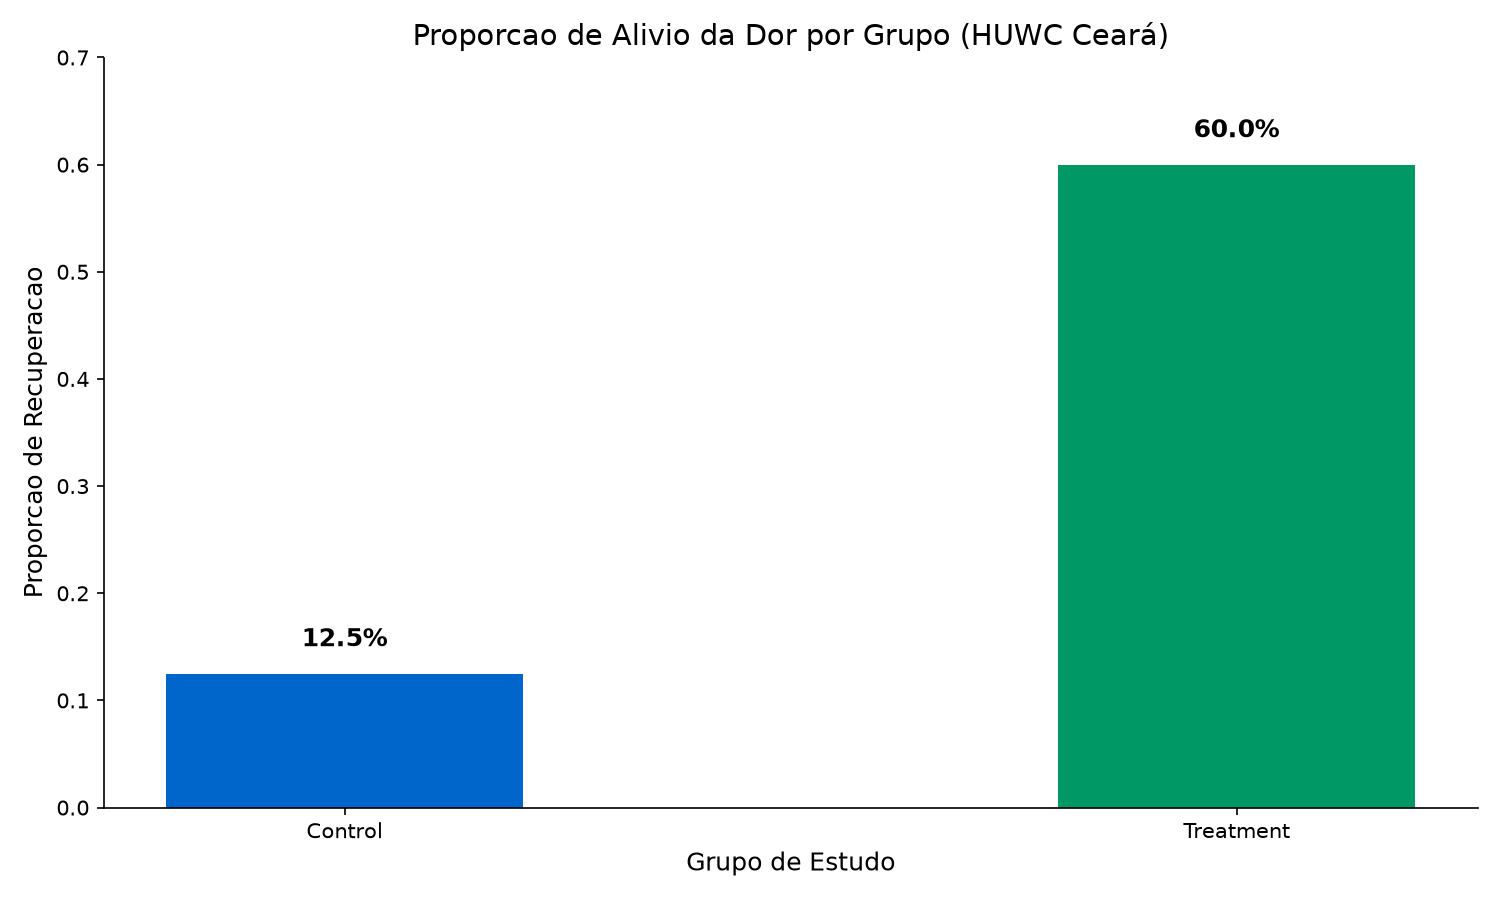
\includegraphics[width=\textwidth]{02_causalidade_barras.png}
        \end{column}
    \end{columns}
\end{frame}

\section{Resultados Potenciais e Hipóteses}

\begin{frame}{Resultados Potenciais (Potential Outcomes)}
    \begin{block}{O que aconteceria se...}
        Antes da divisão do sorteio, cada paciente possui dois resultados potenciais:
        \begin{enumerate}
            \item O resultado obtido caso fosse sorteado para o grupo de tratamento.
            \item O resultado obtido caso fosse sorteado para o grupo de controle.
        \end{enumerate}
    \end{block}
    \begin{block}{A Metáfora do Bilhete de Dois Lados}
        Imagine que cada um dos $31$ pacientes possui um bilhete. O lado esquerdo é a sua melhora com BTA, e o lado direito é sua melhora com salina.
        \begin{itemize}
            \item Para os 15 sorteados no tratamento, revelamos a face esquerda (BTA).
            \item Para os 16 sorteados no controle, revelamos a face direita (salina).
            \item A outra metade de cada bilhete permanece eternamente \textbf{desconhecida}.
        \end{itemize}
    \end{block}
    \centering
    \textit{Nosso desafio estatístico é comparar duas distribuições tendo acesso apenas a metade dos dados de cada bilhete.}
\end{frame}

\begin{frame}{As Hipóteses do Teste Clínico}
    \begin{block}{Hipótese Nula ($H_0$): O Modelo do Acaso}
        A distribuição de todos os $31$ resultados potenciais sob o tratamento é idêntica à distribuição sob o controle. A Toxina Botulínica Tipo A (BTA) não difere do soro fisiológico.
        \begin{itemize}
            \item Sob $H_0$, as faces esquerda e direita do bilhete de cada paciente têm o mesmo valor.
            \item Qualquer diferença observada deve-se puramente ao acaso do sorteio dos grupos.
        \end{itemize}
    \end{block}
    \begin{block}{Hipótese Alternativa ($H_1$): A Presença de Efeito}
        A distribuição de resultados potenciais sob o tratamento é diferente daquela sob o controle. O remédio realmente causa um efeito diferente de um placebo.
    \end{block}
\end{frame}

\section{Estatística de Teste e Simulação de Permutação}

\begin{frame}{Estatística de Teste: Distância de Proporções}
    \begin{block}{Definição da Estatística}
        Para testar a diferença entre os grupos, usamos a distância absoluta (valor absoluto da diferença) entre as proporções de melhora dos dois grupos:
        $$\text{Estatística de Teste} = |p_{\text{tratamento}} - p_{\text{controle}}|$$
    \end{block}
    \begin{block}{Cálculo Observado na Amostra}
        Com base nos dados coletados no HUWC Ceará:
        \begin{itemize}
            \item Proporção de melhora no Tratamento ($p_{\text{tratamento}}$): $9/15 = 0.600$ ($60.0\%$)
            \item Proporção de melhora no Controle ($p_{\text{controle}}$): $2/16 = 0.125$ ($12.5\%$)
            \item Distância Observada:
                $$|0.600 - 0.125| = 0.475 \quad (47.5\%)$$
        \end{itemize}
    \end{block}
    \centering
    \textit{Valores grandes da estatística de teste indicam desvios do modelo do acaso e apoiam a hipótese alternativa ($H_1$).}
\end{frame}

\begin{frame}{Embaralhando Rótulos sob a Hipótese Nula}
    \begin{block}{A Lógica da Simulação}
        Se a hipótese nula $H_0$ é verdadeira, o tratamento não tem efeito. Ou seja, os $11$ pacientes que melhoraram teriam melhorado de qualquer forma, não importando a qual grupo foram alocados.
    \end{block}
    \begin{block}{Algoritmo do Teste de Permutação}
        1. Junte todos os $31$ resultados ($11$ sucessos, $20$ insucessos).
        2. Embaralhe aleatoriamente esses resultados (simulando que os rótulos de grupo foram sorteados novamente).
        3. Separe o vetor embaralhado em um grupo de 16 (Controle) e outro de 15 (Tratamento).
        4. Calcule a nova estatística de teste (distância absoluta).
        5. Repita o processo $20.000$ vezes para obter a distribuição nula.
    \end{block}
\end{frame}

\begin{frame}[fragile]{Código em Python: Teste de Permutação (BTA)}
\begin{lstlisting}[language=Python]
import numpy as np

# Dados: 11 sucessos (1) e 20 fracassos (0)
resultados = np.array([1]*11 + [0]*20)
tamanho_controle = 16
tamanho_tratamento = 15
distancias_simuladas = []

np.random.seed(42)
for _ in range(20000):
    # Embaralha os resultados (rotulos sao fixos)
    embaralhado = np.random.permutation(resultados)
    
    sim_controle = embaralhado[:tamanho_controle]
    sim_tratamento = embaralhado[tamanho_controle:]
    
    # Calcula a diferenca absoluta das proporcoes
    prop_c = np.mean(sim_controle)
    prop_t = np.mean(sim_tratamento)
    distancias_simuladas.append(np.abs(prop_t - prop_c))

# Calcula o P-valor empirico
obs_dist = np.abs(0.60 - 0.125)
p_valor = np.count_nonzero(distancias_simuladas >= obs_dist) / 20000
print(f"P-valor: {p_valor:.5f}")
# Saida esperada: 0.00910
\end{lstlisting}
\end{frame}

\section{Tomada de Decisão e Relação de Causalidade}

\begin{frame}{Tomada de Decisão Visual}
    \begin{columns}
        \begin{column}{0.5\textwidth}
            \textbf{Análise do Histograma Nulo:}
            \begin{itemize}
                \item O histograma mostra os valores da estatística de teste esperados sob a hipótese nula $H_0$.
                \item O valor observado de $0.475$ está marcado com a linha tracejada vermelha.
                \item Apenas uma proporção muito pequena das permutações (dourado) resultou em diferenças maiores ou iguais à observada.
                \item O desvio é muito extremo para ser explicado pelo acaso.
            \end{itemize}
        \end{column}
        \begin{column}{0.5\textwidth}
            \centering
            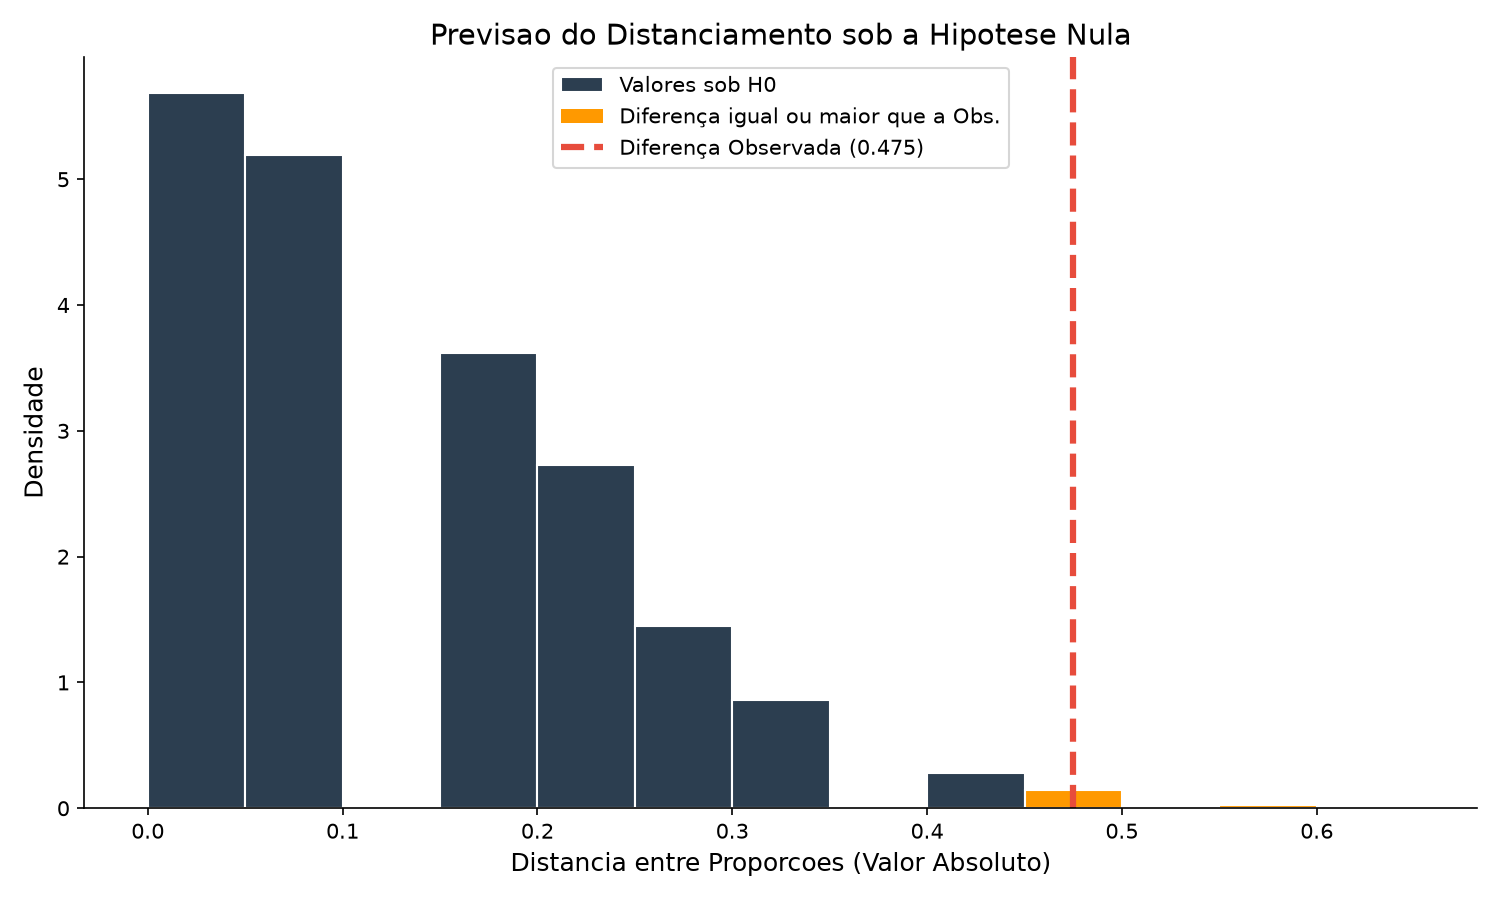
\includegraphics[width=\textwidth]{01_causalidade_histograma.png}
        \end{column}
    \end{columns}
\end{frame}

\begin{frame}{Decisão Estatística e Causalidade}
    \begin{block}{Resultado do Teste no Ceará}
        \begin{itemize}
            \item P-valor empírico calculado: $0.0091$ ($0.91\%$).
            \item Regra de Decisão: Como o P-valor ($0.91\%$) é menor que o nível de significância convencional ($\alpha = 5\%$), \textbf{rejeitamos a hipótese nula $H_0$}.
            \item As evidências estatísticas sustentam a hipótese alternativa $H_1$.
        \end{itemize}
    \end{block}
    \begin{alertblock}{Inferência de Causalidade}
        Como a alocação dos 31 pacientes aos grupos Tratamento e Controle foi feita de forma estritamente aleatória (por sorteio), concluímos que o tratamento com Toxina Botulínica Tipo A (BTA) \textbf{causou} a melhora clínica nos pacientes.
    \end{alertblock}
    \centering
    \textit{A randomização distribuiu as variáveis ocultas igualmente entre os grupos, eliminando o confundimento e validando a relação de causa e efeito!}
\end{frame}

\section{Meta-Análise, Resumo e Referências}

\begin{frame}{Meta-Análise: Uma Visão Cética e Saudável}
    \begin{block}{O Limite da Amostra Pequena}
        Nossos resultados provam causalidade para os $31$ pacientes específicos que participaram do estudo. Mas e para a população geral de pacientes?
    \end{block}
    \begin{block}{A Meta-Análise de 2011}
        Pesquisadores reuniram todos os estudos mundiais de Toxina Botulínica para dor lombar crônica.
        \begin{itemize}
            \item $19$ estudos foram excluídos devido à falta de randomização ou dados incompletos.
            \item Apenas $3$ estudos controlados aleatórios restaram (incluindo o que analisamos).
            \item \textbf{Conclusão:} As evidências clínicas acumuladas ainda são classificadas como de \textbf{baixa qualidade}. Mais pesquisas com amostras maiores são fundamentais antes de uma recomendação de larga escala.
        \end{itemize}
    \end{block}
\end{frame}

\begin{frame}{O Trabalho do Cientista de Dados}
    \begin{block}{O Rigor da Ciência de Dados}
        Qualquer ciência (inclusive a nova ``ciência de dados'') é um caminho complexo que exige rigor analítico e ética na interpretação.
    \end{block}
    \begin{block}{Nosso Repertório de Ferramentas}
        \begin{itemize}
            \item Até o momento, aprendemos apenas uma ferramenta básica: testes de hipóteses via permutação e bootstrap.
            \item Existem limitações claras nos testes clássicos, mas se bem interpretados, oferecem bases sólidas de decisão.
            \item \textbf{Próximos Passos (Olhando para o Futuro):} Após a avaliação, expandiremos nossas capacidades com modelos preditivos:
            \begin{itemize}
                \item \textbf{Regressão:} Previsão de valores contínuos.
                \item \textbf{Classificação:} Atribuição de rótulos categóricos.
            \end{itemize}
        \end{itemize}
    \end{block}
    \centering
    \textit{Lembre-se: não seja o profissional de uma ferramenta só!}
\end{frame}

\begin{frame}{O Caso da Cloroquina: O Perigo da Falta de Randomização}
    \begin{columns}
        \begin{column}{0.55\textwidth}
            \begin{block}{O Erro de Randomização}
                Os autores do famoso estudo sobre cloroquina e azitromicina admitiram: \textbf{o estudo não foi randomizado}.
            \end{block}
            \begin{itemize}
                \item \textbf{Falta de Sorteio:} Os pacientes escolheram se tomavam ou não a medicação, gerando um grave viés de seleção.
                \item \textbf{Consequência:} Sem randomização, premissas de causalidade caem por terra.
                \item \textbf{Consenso Posterior:} Estudos subsequentes robustos confirmaram a ineficácia do tratamento.
            \end{itemize}
        \end{column}
        \begin{column}{0.45\textwidth}
            \centering
            
\includegraphics[width=\textwidth]{estudo_cloroquina.png}
            \vspace{0.1cm}
            \tiny{Título do artigo demonstrando a natureza não-randomizada (\textit{open-label non-randomized}).}
        \end{column}
    \end{columns}
\end{frame}

\begin{frame}{Método Científico}
    \begin{itemize}
        \item O arcabouço de testes de hipóteses é uma ótima ferramenta para a ciência no geral.
        \item Afinal, testar hipóteses é o grande objetivo da ciência!
        \item Note que nem toda Ciência vai usar Estatística ou Ciência de Dados.
        \item Existem várias formas de fazer experimentos/métodos:
        \begin{itemize}
            \item \textbf{Experimentos Físicos:} Equações para explicar o nosso mundo comprovadas via experimentos.
            \item \textbf{Qualitativos:} Estudos onde não necessariamente usamos dados ou médias, mas que ainda assim são feitos com \textbf{método}.
            \item \textbf{Tentativas de Provas para os Teóricos:} Cada tentativa de prova matemática é uma hipótese, por exemplo.
        \end{itemize}
    \end{itemize}
\end{frame}

\begin{frame}{Ciência de Dados no mundo da Ciência}
    \begin{block}{A Incerteza nos Dados}
        ``All datasets involve uncertainty. There may be uncertainty about how they were collected, how they were measured, or the process that created them. Statistical modeling helps quantify and reason about uncertainties in a systematic way.''
    \end{block}
    \begin{alertblock}{Conclusão Importante}
        A Ciência de Dados \textbf{não é toda a ciência}! Ela apenas \textbf{ajuda no método científico} ao fornecer uma forma sistemática de analisar dados e quantificar incertezas.
    \end{alertblock}
\end{frame}

\begin{frame}{O Ciclo do Método Científico}
    O avanço da ciência baseia-se em um ciclo sistemático e replicável:
    \begin{block}{As Fases do Ciclo:}
        \begin{enumerate}
            \item \textbf{Pergunta:} Formulada de maneira clara (ex: Fumar na gestação afeta o peso do recém-nascido?).
            \item \textbf{Revisão de Literatura:} Investigar o que a comunidade científica já descobriu sobre o assunto.
            \item \textbf{Hipótese:} Definir o modelo nulo ($H_0$) e a alternativa de efeito ($H_1$).
            \item \textbf{Experimento:} Testes A/B aleatórios são fundamentais para gerar dados confiáveis.
            \item \textbf{Análise do Resultado:} Avaliação da significância e do tamanho do efeito.
            \item \textbf{Comunicação:} Publicar os resultados com os métodos claros para permitir a replicação.
        \end{enumerate}
    \end{block}
\end{frame}

\begin{frame}{A Replicação como Regra de Ouro}
    \begin{block}{Se não é replicável, não é ciência!}
        \begin{itemize}
            \item Um único experimento com resultado positivo (como BTA para dor lombar com $N=31$) não é definitivo.
            \item Existe sempre uma chance de erro estatístico ou viés na amostra local.
            \item Um novo experimento, sob as mesmas hipóteses e feito por outro pesquisador, deve ser capaz de reproduzir o efeito.
        \end{itemize}
    \end{block}
    \begin{block}{Meta-Análise}
        O estudo que consolida os resultados de múltiplos experimentos independentes. É a meta-análise que estabelece o consenso científico final sobre a eficácia de um tratamento.
    \end{block}
\end{frame}

\begin{frame}{Críticas aos Testes de Hipóteses e P-valores}
    \begin{block}{A Crítica ao Limiar dos 5\%}
        Há um movimento de estatísticos e cientistas contra o uso mecânico e cego da regra de significância de $p < 0.05$.
        \begin{itemize}
            \item Críticos apontam problemas de ``P-hacking'' (manipulação de dados até obter P-valor significativo) e o viés de publicação.
            \item Um P-valor sozinho não mede a força da evidência ou a importância prática de um resultado.
        \end{itemize}
    \end{block}
    \begin{alertblock}{O que relatar em seus estudos?}
        Para garantir o rigor, sempre apresente: (1) O valor exato do P-valor, (2) O tamanho amostral ($N$), (3) O tamanho do efeito (effect size) e (4) Como testou (ex: Bootstrap vs. Permutação).
    \end{alertblock}
\end{frame}

\begin{frame}{Resumo e Principais Aprendizados}
    \begin{block}{Ideias Fundamentais da Aula}
        \begin{itemize}
            \item \textbf{Causalidade vs. Associação:} Experimentos Controlados Aleatórios (RCTs) neutralizam fatores de confundimento, permitindo comprovar causa e efeito.
            \item \textbf{Resultados Potenciais:} A conceituação imaginária de todos os cenários possíveis para cada indivíduo (metáfora do bilhete).
            \item \textbf{Teste de Permutação:} O embaralhamento computacional de rótulos simula o acaso sob a hipótese nula $H_0$.
            \item \textbf{P-valor Empírico:} Permite determinar se a diferença observada é comum ou extremamente improvável sob o acaso.
            \item \textbf{Método Científico:} Rigor, replicação e pensamento crítico são fundamentais na análise de dados.
        \end{itemize}
    \end{block}
\end{frame}

\begin{frame}{Referências Bibliográficas}
    \begin{block}{Leituras Recomendadas}
        \footnotesize
        \begin{itemize}
            \item \textbf{Learning Data Science} \\
            Sam Lau, Joey Gonzalez, and Deb Nolan. \\
            Capítulo 17: Inference, Prediction, and Generalization. \\
            \url{https://learningds.org/ch/17/inf_pred_gen_HT.html}
            \vspace{0.3cm}
            \item \textbf{Computational and Inferential Thinking} \\
            Ani Adhikari and John DeNero. \\
            Capítulo 11: Testing Hypotheses (Seção 11.1 - Causality). \\
            \url{https://inferentialthinking.com/chapters/11/testing-hypotheses/}
        \end{itemize}
    \end{block}
\end{frame}


\end{document}
